\documentclass[%
12pt, %
final, % 
oneside, % 
onecolumn, %  
centertags]{article} % относится к классу article и размер шрифта 12 пунктовб, {article: статья, report: отчеты и диссертации, book: книга, letter: письмо}

% \usepackage{fontspec}
 
% \setmainfont{Times New Roman}

% \documentclass[a4paper, 12pt]{report}

\topmargin= -30pt % насколько сверху будет страница
\textheight= 650pt


\usepackage[utf8]{inputenc} % задает кодировку, utf-8 кодировка, включающая в себя знаки почти всех языков мира
\usepackage[english]{babel} % подключает необходимые языки, основным языком является английский

\selectlanguage{english} % настройки будут на английском, но писать будет на русском

\usepackage{euscript}
\usepackage{supertabular}

\renewcommand{\baselinestretch}{1.0} 

\usepackage[colorlinks=true,linkcolor=blue,unicode=true,urlcolor = blue]{hyperref} %hypered
\usepackage[pdftex]{graphicx} % для графики

\usepackage{amsthm, amssymb, amsmath, amsfonts} % математический пакет, математические шрифты
\usepackage{textcomp}
\usepackage[noend]{algorithmic}
\usepackage[ruled]{algorithm}
\usepackage{lipsum}
\usepackage{indentfirst}
\usepackage{babel}
\usepackage{pgfplots}
\usepackage{setspace}
\usepackage{xcolor}
\usepackage{hyperref}
\usepackage{subfigure}

\setcounter{secnumdepth}{5}
\setcounter{tocdepth}{5}
\newcommand\simpleparagraph[1]{%
  \stepcounter{paragraph}\paragraph*{\theparagraph\quad{}#1}}



\linespread{1.0} 
\setlength{\parindent}{2.4em}
\setlength{\parskip}{0.1em}

\pgfplotsset{compat=1.9}
\pgfplotsset{model/.style = {blue, samples = 100}} 
\pgfplotsset{experiment/.style = {red}}

\theoremstyle{plain}
\binoppenalty=10000

% \newtheorem{theorem}{Теорема}[section] % theorem

\theoremstyle{definition}
% \newtheorem{definition}{Определение}[subsection]
\newtheorem{definition}{Definition}[subsection]

\theoremstyle{remark}
% \newtheorem{remark}{Замечание}[section]

% \newtheorem{corollary}{Следствие}

% \newtheorem{proposition}{Proposition}

% \newtheorem{example}{Пример}

% \newtheorem{lemma}{Лемма}[section]

\renewcommand*{\proofname}{Proof}

\graphicspath{ {./images/} }


% \usepackage{amsmath,amsfonts,amssymb, setspace}  % Разнообразные математические команды и значки
% \usepackage{indentfirst}     % Отступ в первом абзаце

% \pagestyle{empty}
\usepackage[left=2.5cm, right=1.5cm, top=2.5cm, bottom=2.5cm]{geometry}
\usepackage[medium]{titlesec}
\usepackage{graphicx}
% \graphicspath{ {./images/} }

\begin{document}

	\begin{titlepage} 
		\begin{center}
		\textbf{}\\[2.0cm]
		\LARGE FEDERAL STATE AUTONOMOUS EDUCATIONAL INSTITUTION OF HIGHER EDUCATION \\[0.5cm]
		\Large ITMO UNIVERSITY \\[3cm]
		\LARGE Report\\
		\Large on learning practice № 2\\
		\Large Analysis of multivariate random variables \\[4cm]


		\begin{flushright}
		Performed by\\
		Aleksandr Shirokov\\
		Team 26, J4133c\\
		\ \\

		\end{flushright}

		\vfill 

		{\Large {St. Petersburg}} \par
		{\Large {2021}}
		\end{center} 
	\end{titlepage}

\tableofcontents
\newpage

\section{Lab 2}

\subsection{Dataset Info}

For labs we have used a dataset which contains information of bitcion price trend indicators. Before doing task, I will write a small tutorial about how to download and use this dataset:

\begin{enumerate}
	\item Download dataset from this \href{https://www.kaggle.com/devbcdestiller/bitcoin-usdt-price-trend-indicators}{link} and save it in \textsc{./data/} folder with filename \textsc{data.csv}
	\item Apply several feature engineering using code in \textsc{mma\_lab\_2\_shirokov.ipynb} notebook
\end{enumerate}

This dataset contains that columns:

\begin{itemize}
	\item \textsc{Open} - open price
	\item \textsc{Volume} - volume of trading
	\item \textsc{RSI} - indicator RSI
	\item \textsc{MACD Signal} - indicator MACD Signal
	\item \textsc{month} - month number
	\item \textsc{STOCHRSI-D} - indicator STOCH
	\item \textsc{quantile\_Volume} - binned volume
	\item \textsc{Close} - target variable, close price
\end{itemize}

\newpage

\subsection{Plotting a non-parametric estimation of PDF in form of a histogram and Kernel density function for MRV (or probability law in case of discrete MRV).}

Firstly i have visualised a non-parametric estimation of PDF in form of a histogram and Kerner density function on the same plot for each dataset variable, and after that visualised the distribution (scatterplot and non-parametric PDF plus KDE) between every pair of variables (not using categorical). 


\begin{center}
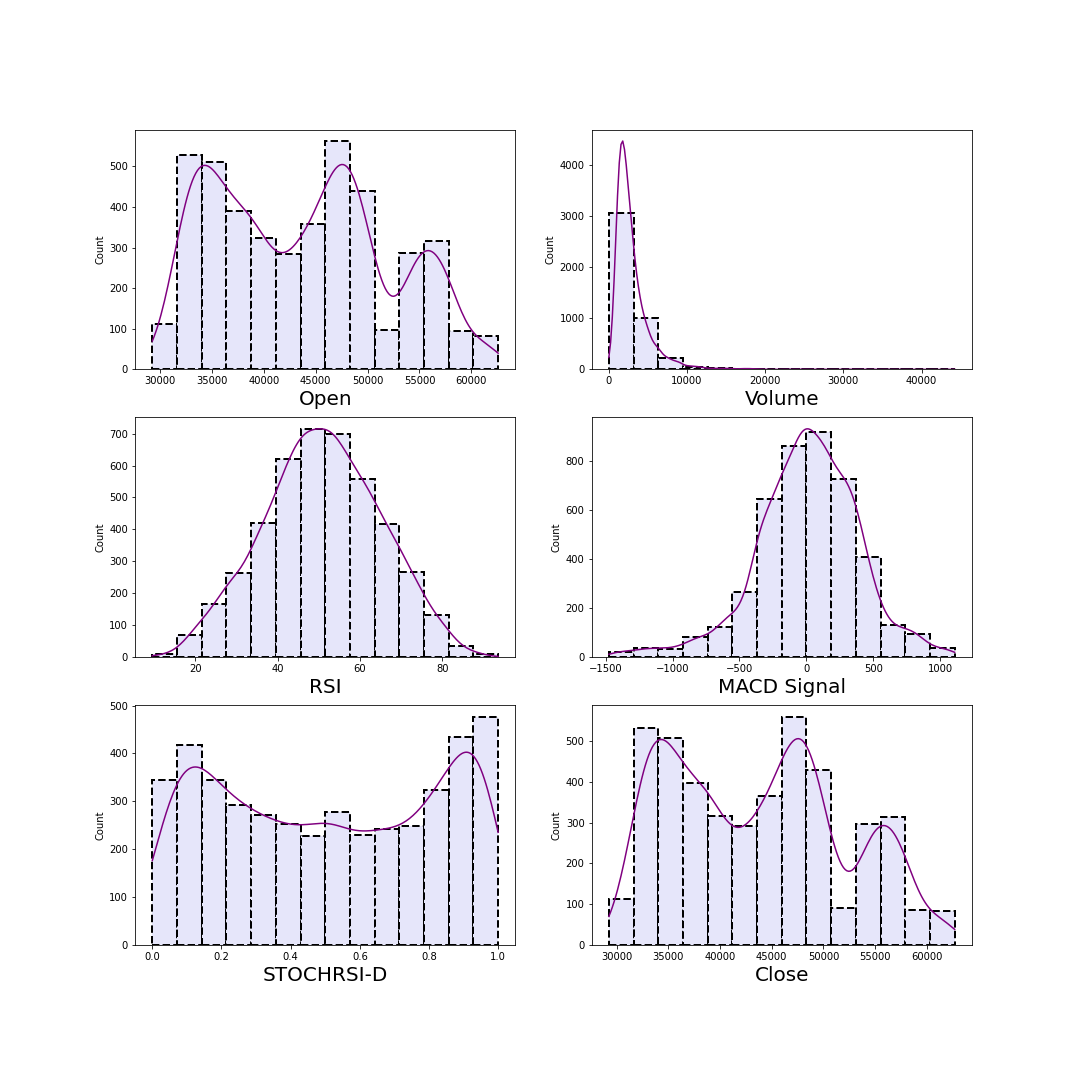
\includegraphics[scale=0.45]{images/task_1_hist.png}

Histogram with bins usin \textsc{Sturges} rule and KDE (default epanechnikov kernel) 
\end{center}

\begin{center}
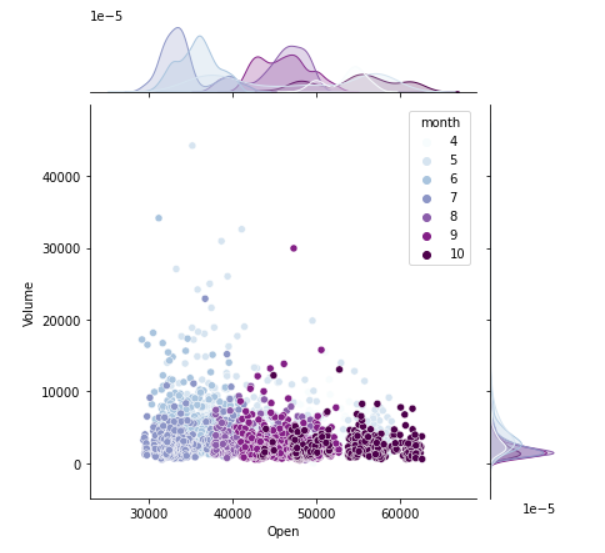
\includegraphics[scale=0.7]{images/mvr_Open_Volume.png}

\end{center}

\begin{center}
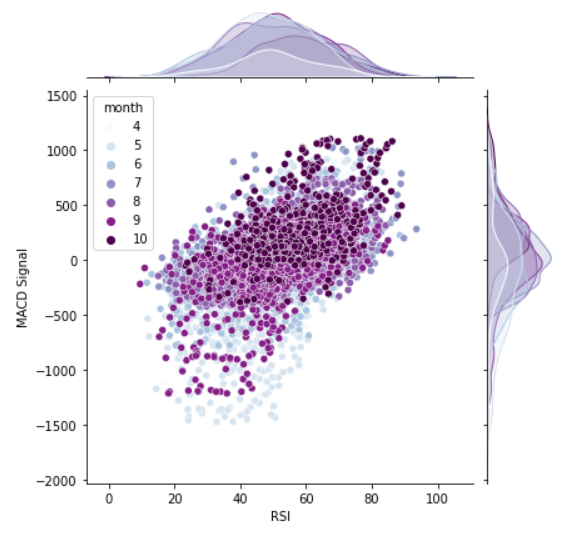
\includegraphics[scale=0.7]{images/mvr_RSI_MACD Signal.png}

Examples of distribution between pairs of variables with \textsc{hue=month}
\end{center}

Every plot was visualised using python package \textbf{Seaborn}.

\subsection{Estimation of multivariate mathematical expectation and variance.}

In this subsection I have counted the mathematical statistic of expectation and variance using methods of \textsc{pandas.DataFrame} - \textsc{mean()} and \textsc{var()}.

\begin{center}
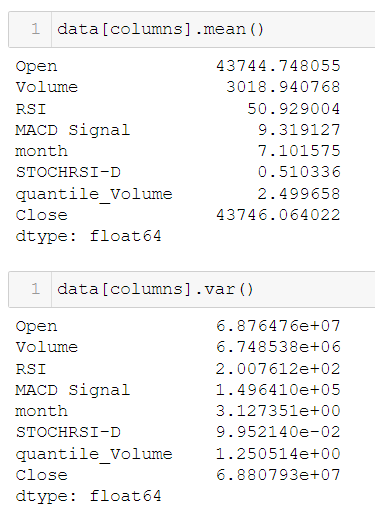
\includegraphics[scale=1]{images/mean_var.png}

The results of subtask 2
\end{center}

\newpage

\subsection{Non-parametric estimation of conditional distributions, mathematical expectations and variances.}

The condition determined the value of the categorical variable, for our dataset this variable is \textsc{quantile\_Volume}. For each \textsc{quantile\_Volume} value, step $1$ has been reproduced and information for every conditional distribution about mean and var has been counted.

\begin{center}
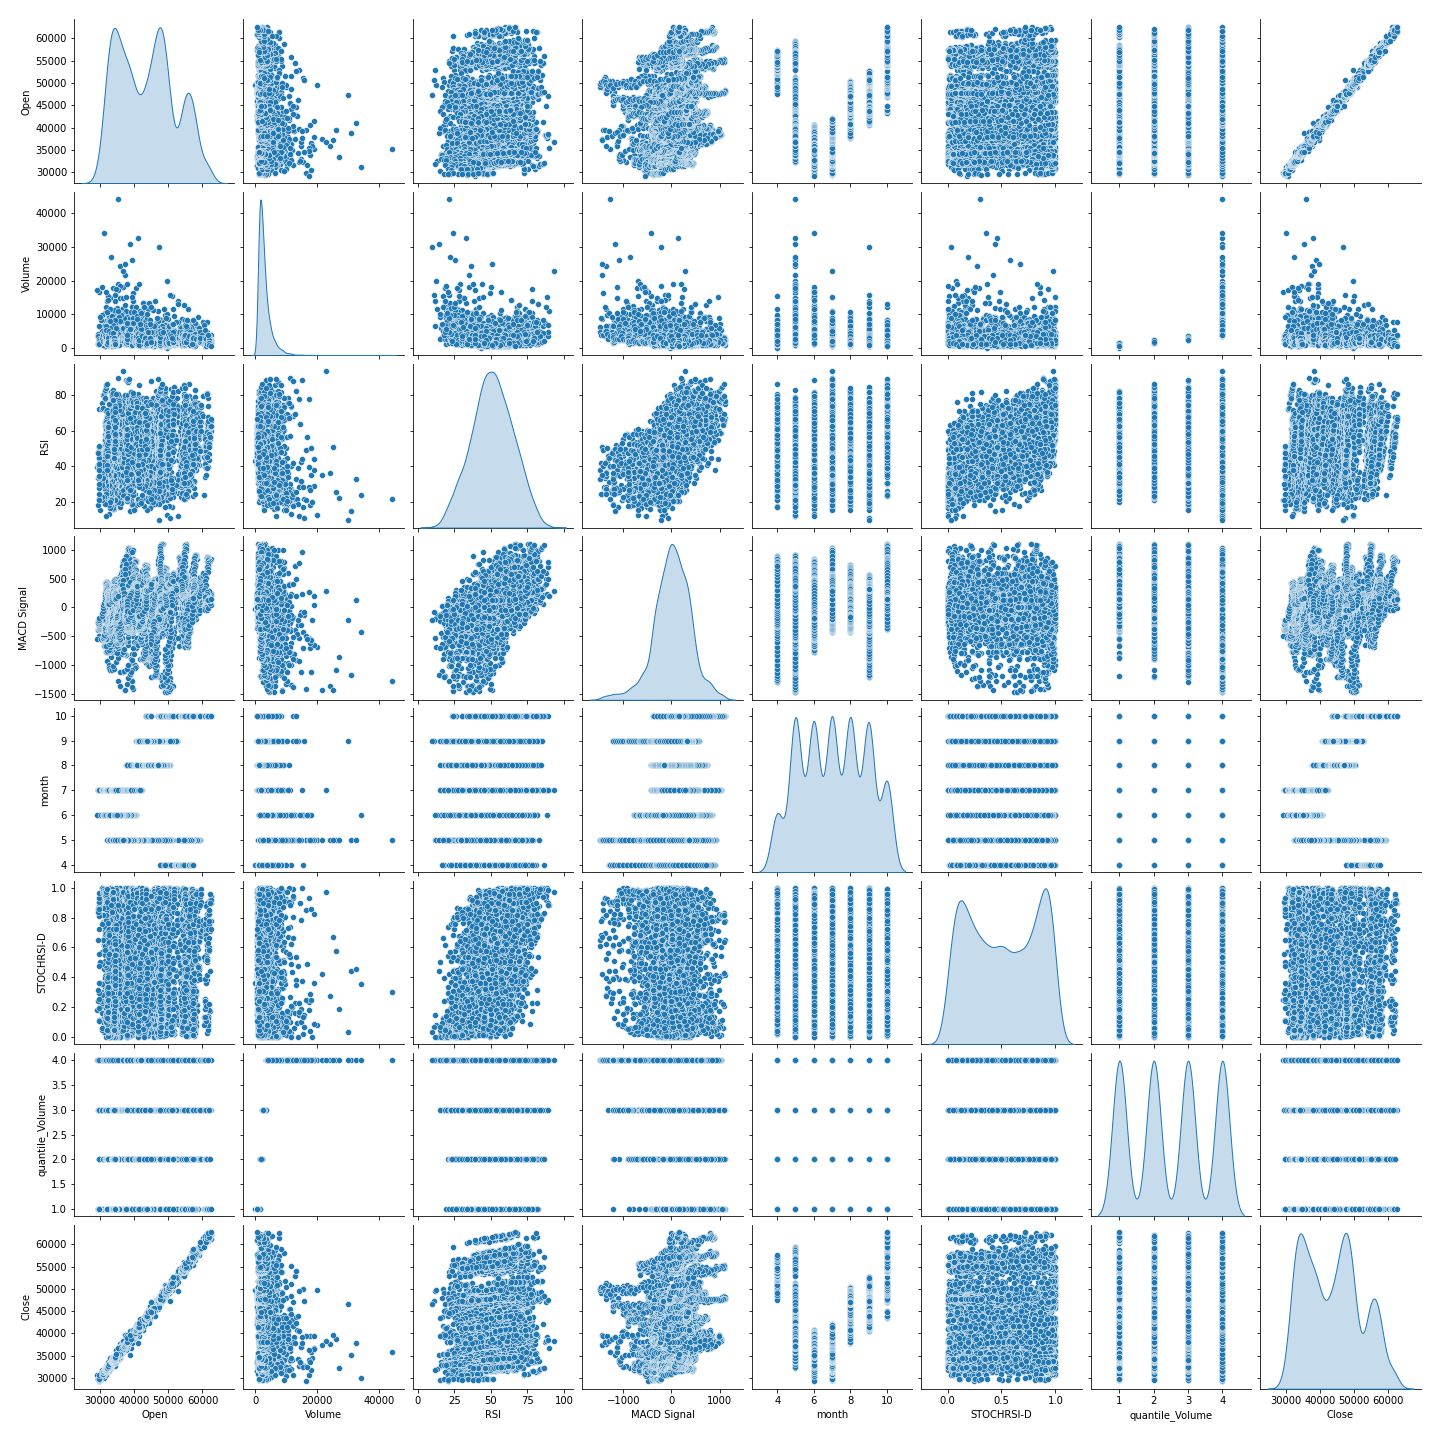
\includegraphics[scale=0.35]{images/distr.png}

Distribution of each pairs of variables
\end{center}

\begin{center}
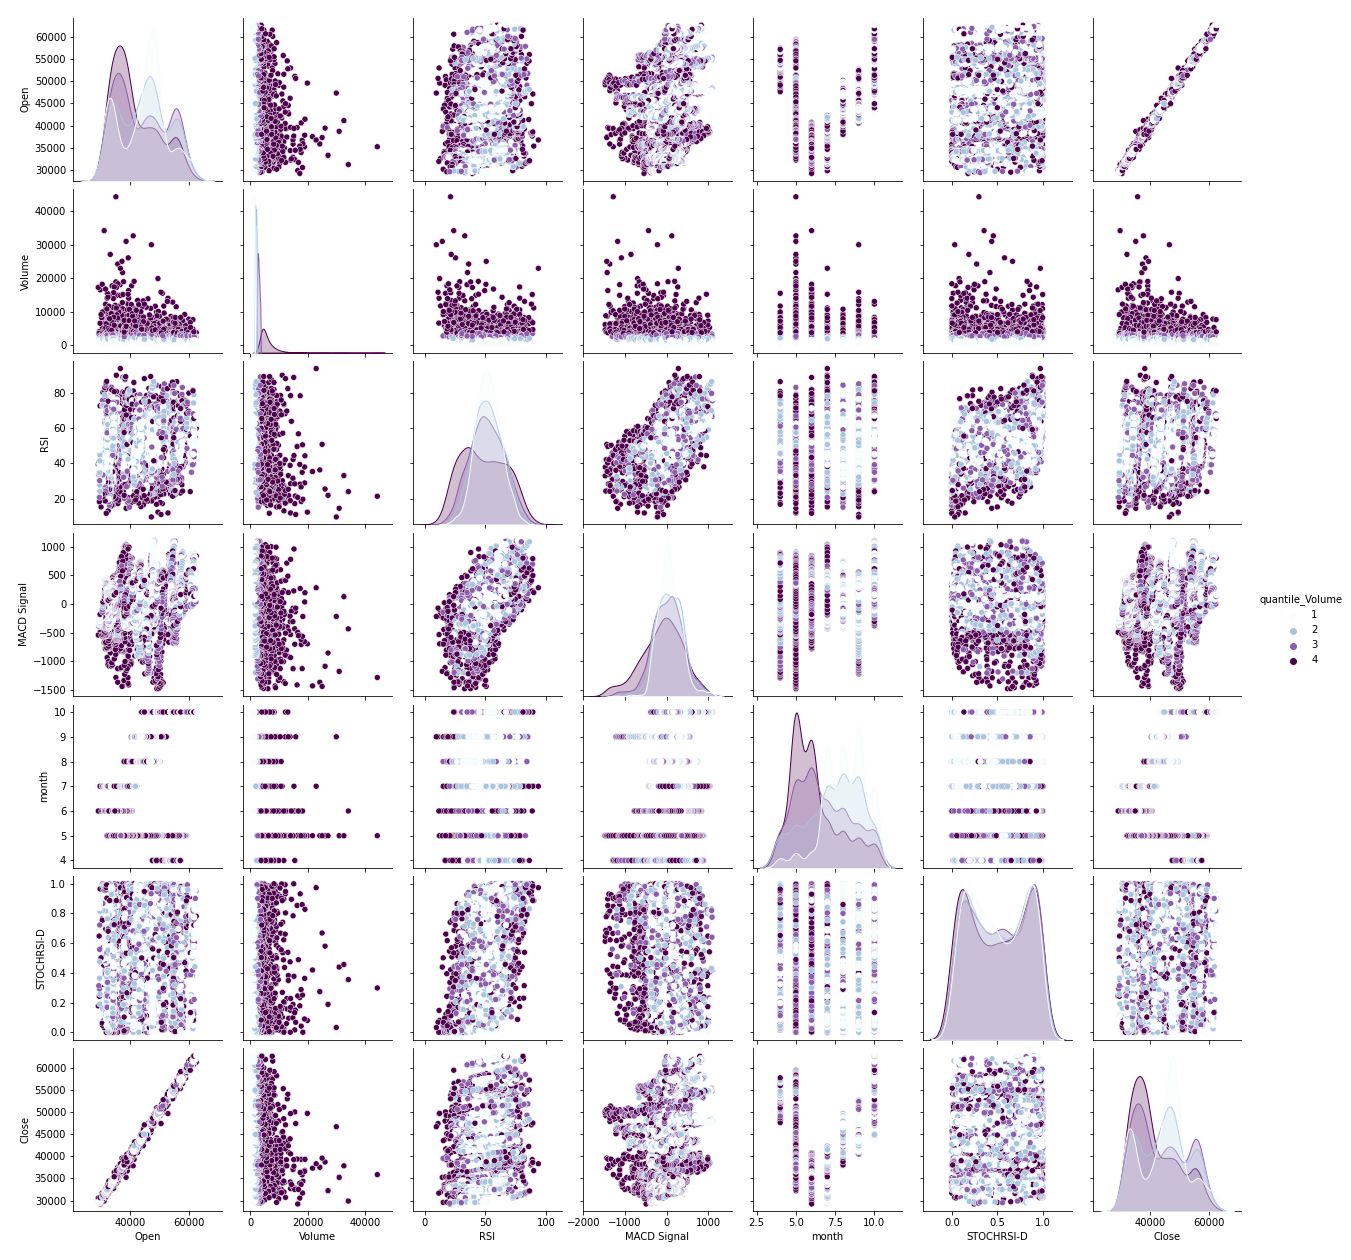
\includegraphics[scale=0.4]{images/distr_hue_quantile_volume.png}

This is distribution of pairs of variables for each cateofry of \textsc{quantile\_Volume} using seaborn method \textsc{seaborn.pairplot}
\end{center}

\begin{center}
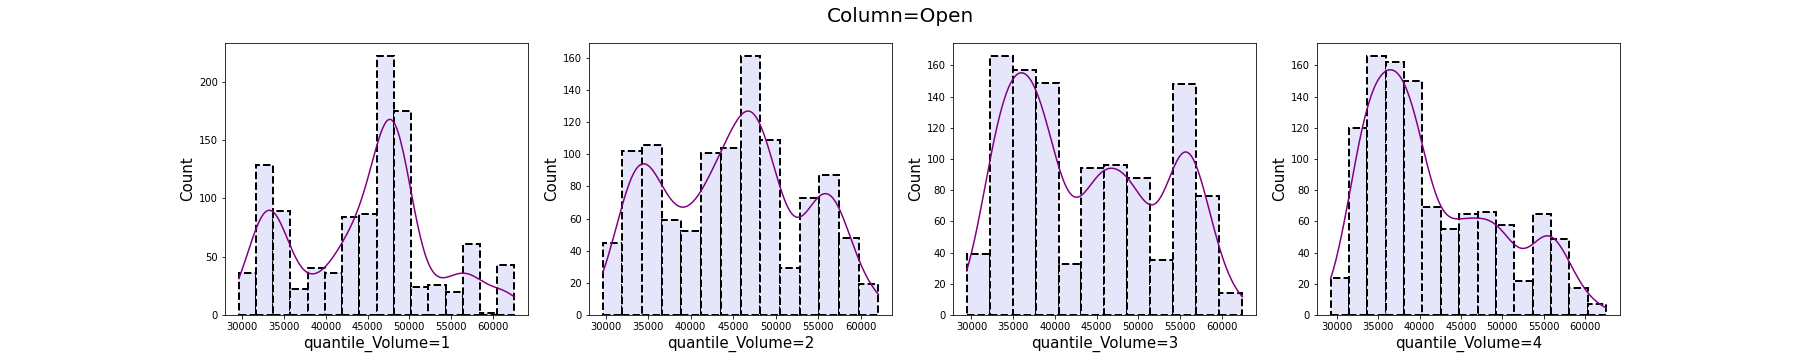
\includegraphics[scale=0.3]{images/conditional_distr_column_Open.png}
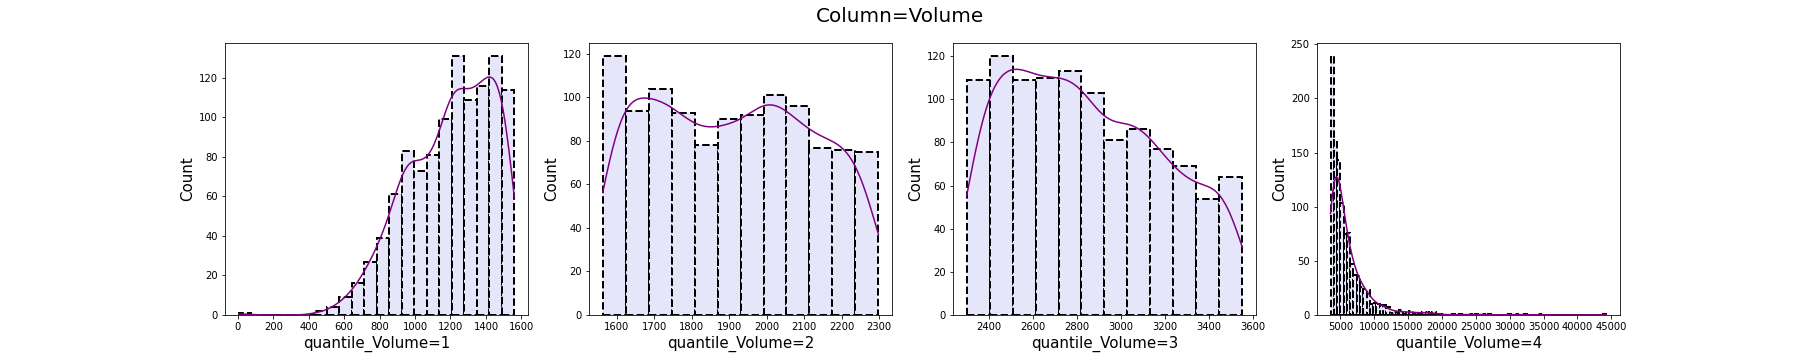
\includegraphics[scale=0.3]{images/conditional_distr_column_Volume.png}
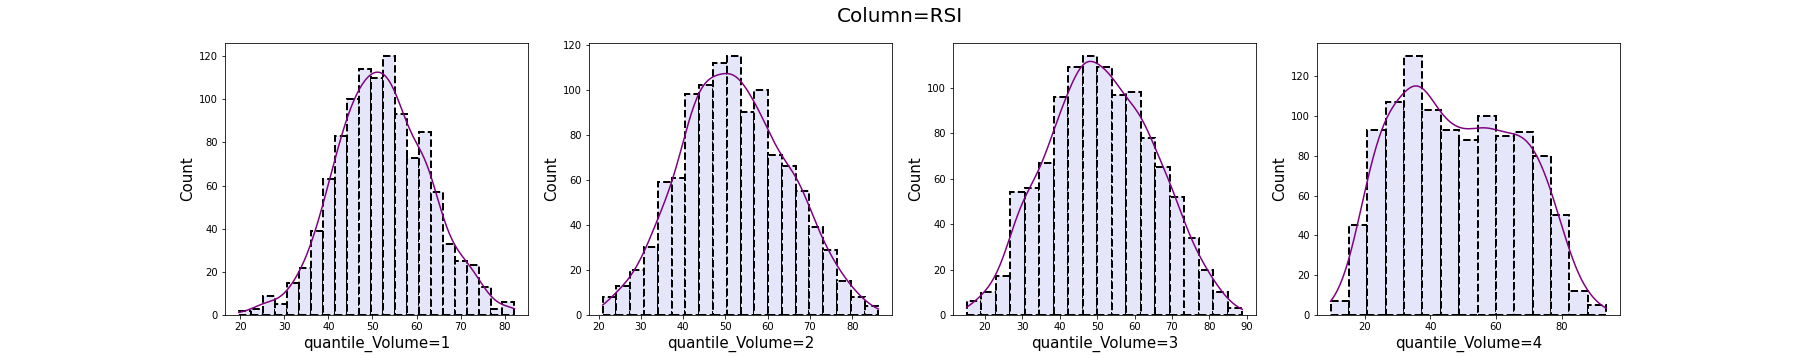
\includegraphics[scale=0.3]{images/conditional_distr_column_RSI.png}
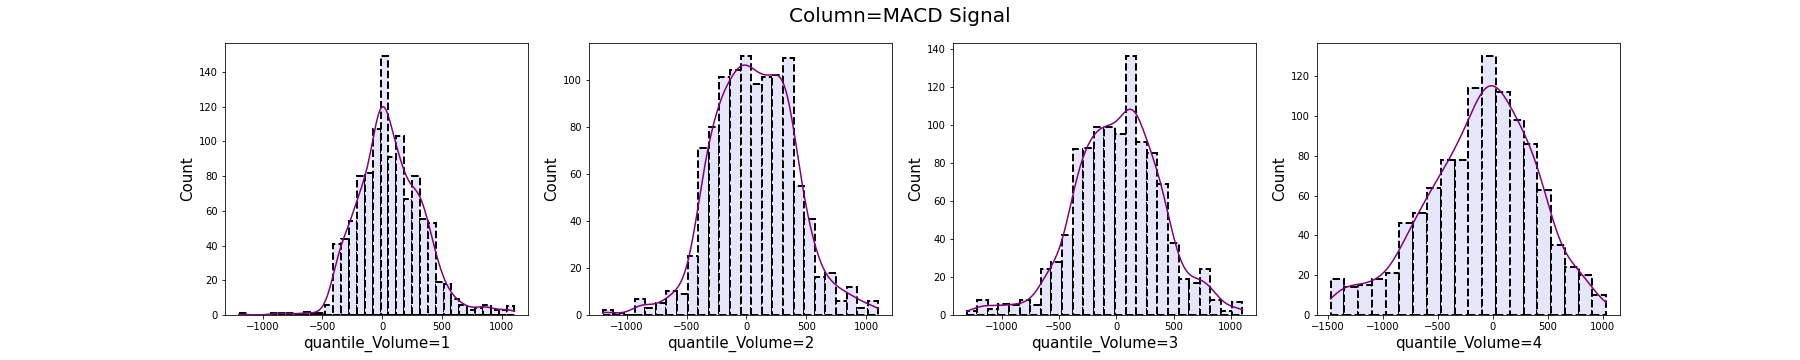
\includegraphics[scale=0.3]{images/conditional_distr_column_MACD Signal.png}
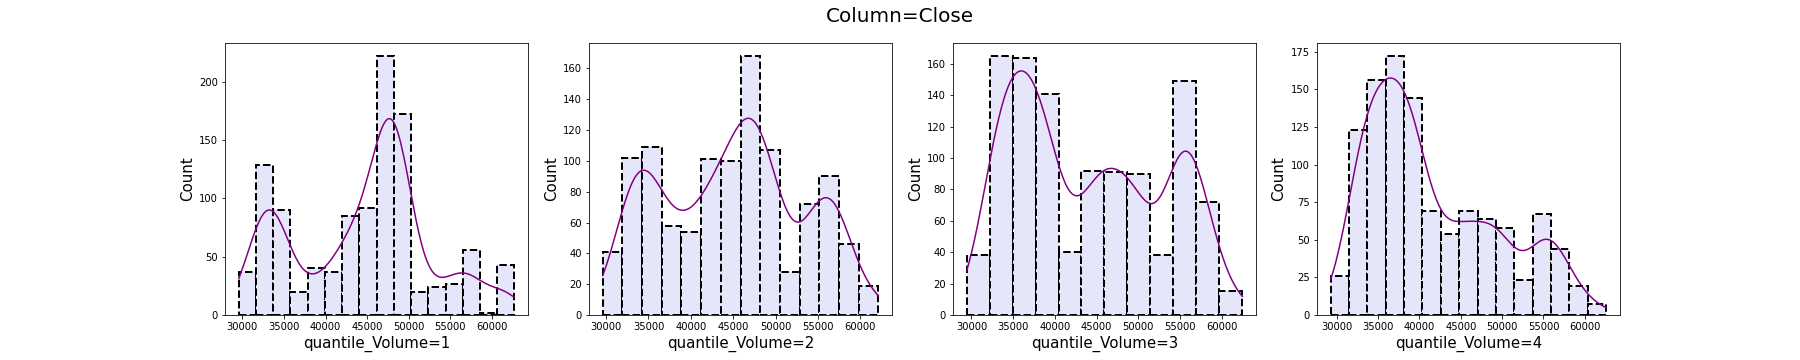
\includegraphics[scale=0.3]{images/conditional_distr_column_Close.png}

Some conditional distributions for each variable, which depends on \textsc{quantile\_Volume}
\end{center}

After I have counted conditional mathematil expectation and variance and visualised it as \textsc{DataFrame}.

\begin{center}
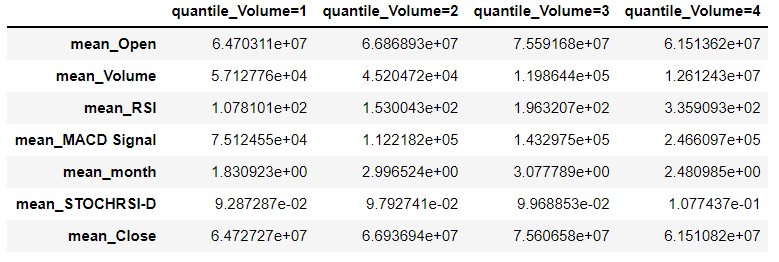
\includegraphics[scale=0.9]{images/cond_mean.png}
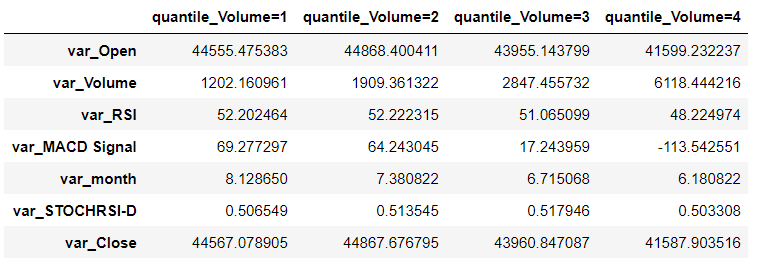
\includegraphics[scale=0.9]{images/cond_var.png}

Conditional mathematical expectation and variance for each value of categorical variable
\end{center}

\newpage

\subsection{Estimation of pair correlation coefficients, confidence intervals for them and significance levels.}

In this task first I have visualised correlation plot using \textsc{sns.heatmap} and after that for each correlation i have counted confidence intervals. To find the numerical characteristics of the confidence intervals, the stats module of the \textsc{SciPy} package was used.

\begin{center}
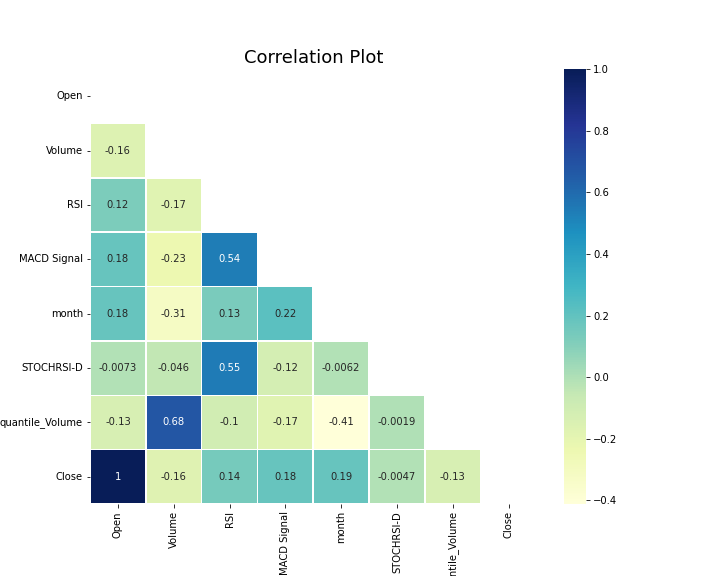
\includegraphics[scale=0.5]{images/correlation_plot.png}

Correlation plot
\end{center}

As we can see on the correlation Plot, column Open has a very high correlation with target value. Other columns have low correlations between each other. For each pair of feature confidence interval of correlation has been counted.

\begin{center}
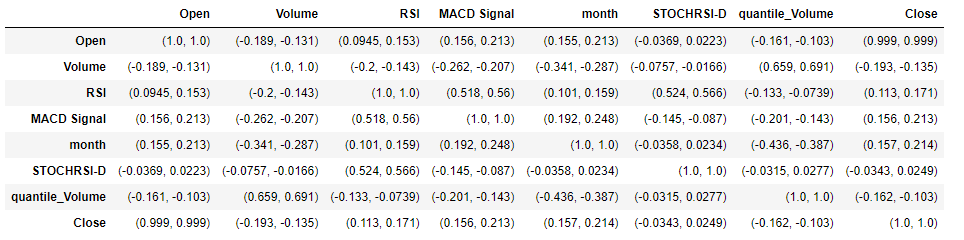
\includegraphics[scale=0.6]{images/corr_coef.png}

Confidence interval of each correlation
\end{center}

\subsection{Task formulation for regression, multivariate correlation.}

Due to results in previous subtask, we will try to predict \textbf{target} column \textsc{target=Close} by \textbf{predictors}:
$$\text{Open}, \text{Volume}, \text{RSI}, \text{MACD Signal}, \text{month}, \text{STOCHRSI-D}, \text{quantile\_Volume}$$

\subsection{Regression model, multicollinearity and regularization (if needed).}

In this task I have used python package \textsc{scikit-learn} and its implementation of \textsc{LinearRegression}, \textsc{Lasso Regression} and \textsc{Ridge} Regression. The cross-validation technique on $10$ folds with differentseeds was used to count a \textit{Mean Absolute Error} (MAE) and \textit{Root Mean Squared Error} (RMSE) to compare results. Te Ridge and Lasso regression was used for regularization cause \textit{OPEN} predictor has very big colleration with target \textit{CLOSE}, so we want to make weights of each predictor be contolled by optimization task. 

For Lasso and Ridge Regression the best $\alpha$ (coefficient of regularization) was found from grid $\alpha_i = [0.001, 1]$. 

Let's see the results.

\begin{center}
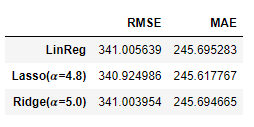
\includegraphics[scale=0.6]{images/results_reg.png}

Results of implementation of each method. The Lasso method with counted value of regularization coefficient $\alpha=0.76$ was the best due to minimizing \textsc{MAE} and \textsc{RMSE} metrics.
\end{center}

\begin{center}
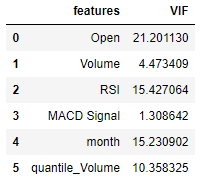
\includegraphics[scale=0.9]{images/vif_data.png}

Also, using \textsc{variance\_inflation\_factor} from \textbf{StatsModels} package the variance inflation factor has been counted. We can see that with \textsc{Open}, \textsc{RSI}, \textsc{month}, and \textsc{quantile\_Volume} multicollinearity is high.
\end{center}

\subsection{Quality analysis.}

\begin{center}
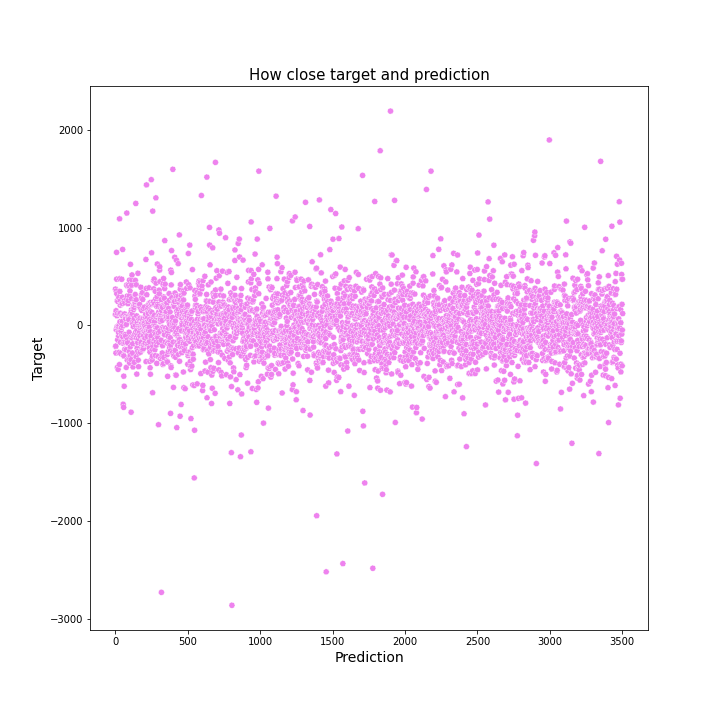
\includegraphics[scale=0.7]{images/target_predict.png}

How close target and prediction
\end{center}

\begin{center}
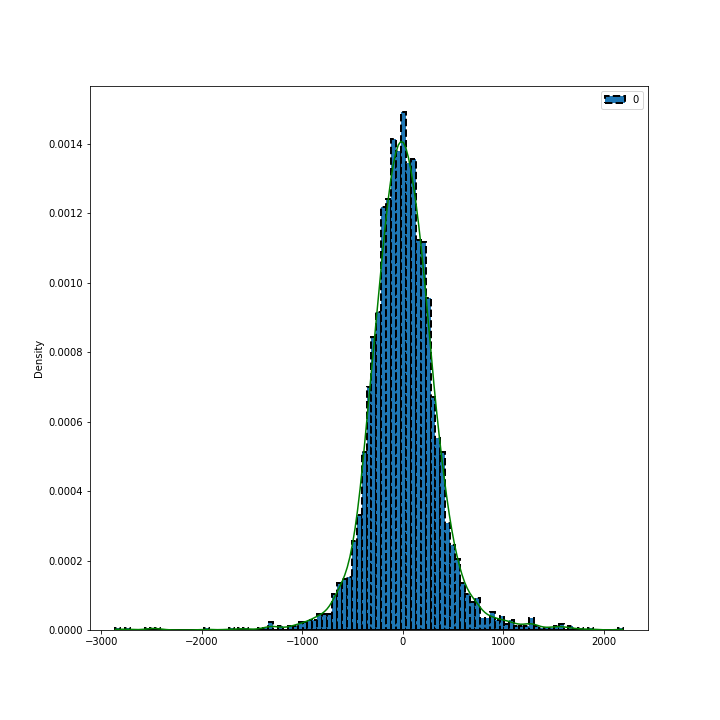
\includegraphics[scale=0.55]{images/residuals.png}

Residuals of model - difference between target and predict.
\end{center}

As you can see in the plot, the model errors have a good normal distribution around $0$. In the future, to improve the quality of the model, one can analyze the instances on which the model makes the most mistakes, and, for example, remove it from the training set.

\section{Source code}

The link to the sourse code which is placed on my \href{https://github.com/aptmess/MMA/}{github}.

\section{Conclusion}

I have learned about some methods of multivariate data analysis, used some popular Python packages, have understood the data of the dataset, used linear regression model with regularization and best coeffecient of refulatization and applied some algorithms of mathematical statistic for calculating confidence interval. 

\end{document}